\chapter{Design}
The development of Flycatcher can be divided into distinct phases, which correspond to the components of the application. In order for the reader to follow and understand the development process, we feel that it is best to start off by giving them a sense of the big picture. Hence, in this chapter we will explain our choice of programming environment, briefly describe the components and give an overview of the system.

\section{Environment}
\subsection{V8 engine}

In picking a JavaScript engine to work with to develop \textsf{Flycatcher}, we looked for the following characteristics:
\begin{itemize}
   \item developer friendliness
   \item a standalone release (many are coupled with browsers)
   \item speed of execution
   \item open source
   \item strong online community
   \item conform to the latest ECMAScript standard, ECMA-262 edition 5
   \item meta-programming features
   \item runs on x86 or x86-64 processors
\end{itemize}

Of the three main contenders in these categories, namely Firefox's SpiderMonkey and Rhino engines and Google's V8, V8 was chosen as it was by far the strongest, notably in terms of execution speed and developer friendliness. The version of V8 used is 3.9.5.

\subsection{Node.js framework}
\begin{figure}[h]
%\hspace*{0.2cm}
\centering

\includegraphics[scale=0.2]{./components/chapter3/nodejs.png}
\end{figure}

JavaScript's debut on the server side prompted the need for a form of application development library support for the language. Thankfully this need was partially met by the development of \emph{Node.js} that started in 2009. Although the framework is intended as an event-driven web framework, the fact that it has a strong online developer community and a variety of valuable open source contributions makes it appealing for developing JavaScript in general. It is all the more appealing to us because it is built on top of the V8 JavaScript engine, which is our engine of choice.

On top of its built-in library support, Node.js offers an efficient package manager \texttt{npm}, which allows us to effectively separate our work into components, as well as easily import plugins from the open source community. The Node.js release used to deveop \textsf{Flycatcher} is version 0.7.5.


\section{Components}
The process of automatically generating tests using the approach we have chosen, dynamic test generation, naturally divides into distinct stages. In this section we will outline and briefly describe what those stages are.

\subsection{Analyser}
The very first task that \textsf{Flycatcher} needs to perform is a dynamic \emph{analysis} of the source code, in order to extract information about the program under test. The \textsf{Analyser} component performs this role: extracting the information that is necessary to even start the test generation process at all. Intuitively, we can think of it as mapping the source code into \textsf{Flycatcher}'s data structures, which are then used in the test generation process.

\subsection{Test Generator}
The next component involved is the \textbf{Test Generator}, which has two implementations consisting of a random test generator to start off with followed by a search-based generator for improved efficiency. Naturally, the more runtime information we have on the class under test (CUT) the more accurate the tests can be. Hence, the initial tests are not accurate but serve to gather runtime information, until we have sufficient information to generate tests with confidence that they are appropriate. As such, this component is tightly coupled with another, which orchestrates a virtual runtime environment in order to collect the necessary runtime information: the \textsf{Executor}.

\subsection{Executor}
The \textsf{Executor} component has two major responsibilities:
\begin{enumerate}
   \item providing a bespoke runtime environment that enables the collection of information concerning the type of the parameters of a method under test (MUT)
   \item tracking the code coverage achieved by the generated tests, in order to measure their quality
\end{enumerate}

The \textsf{Executor} and the \textbf{Test Generator} thus work in to-and-fro until either satisfactory code coverage is achieved or a termination criterion is met. Upon termination, the tests that were deemed accurately typed and that contributed to code coverage are collated into a suite of unit tests and output to the user in a format corresponding to his preferred unit testing framework. The tests that reveal an error in the program under test or a possible mistake made by \textsf{Flycatcher}'s type inference mechanism are also output, as \emph{failing tests}.

\section{System}
Figure \ref{system} gives an idea of the overall system and how the components fit together, so that the reader can appreciate the journey from the program under test to a suite of test cases that can be used for regression unit-testing.

\begin{figure}[h]
\hspace*{-0.3cm}
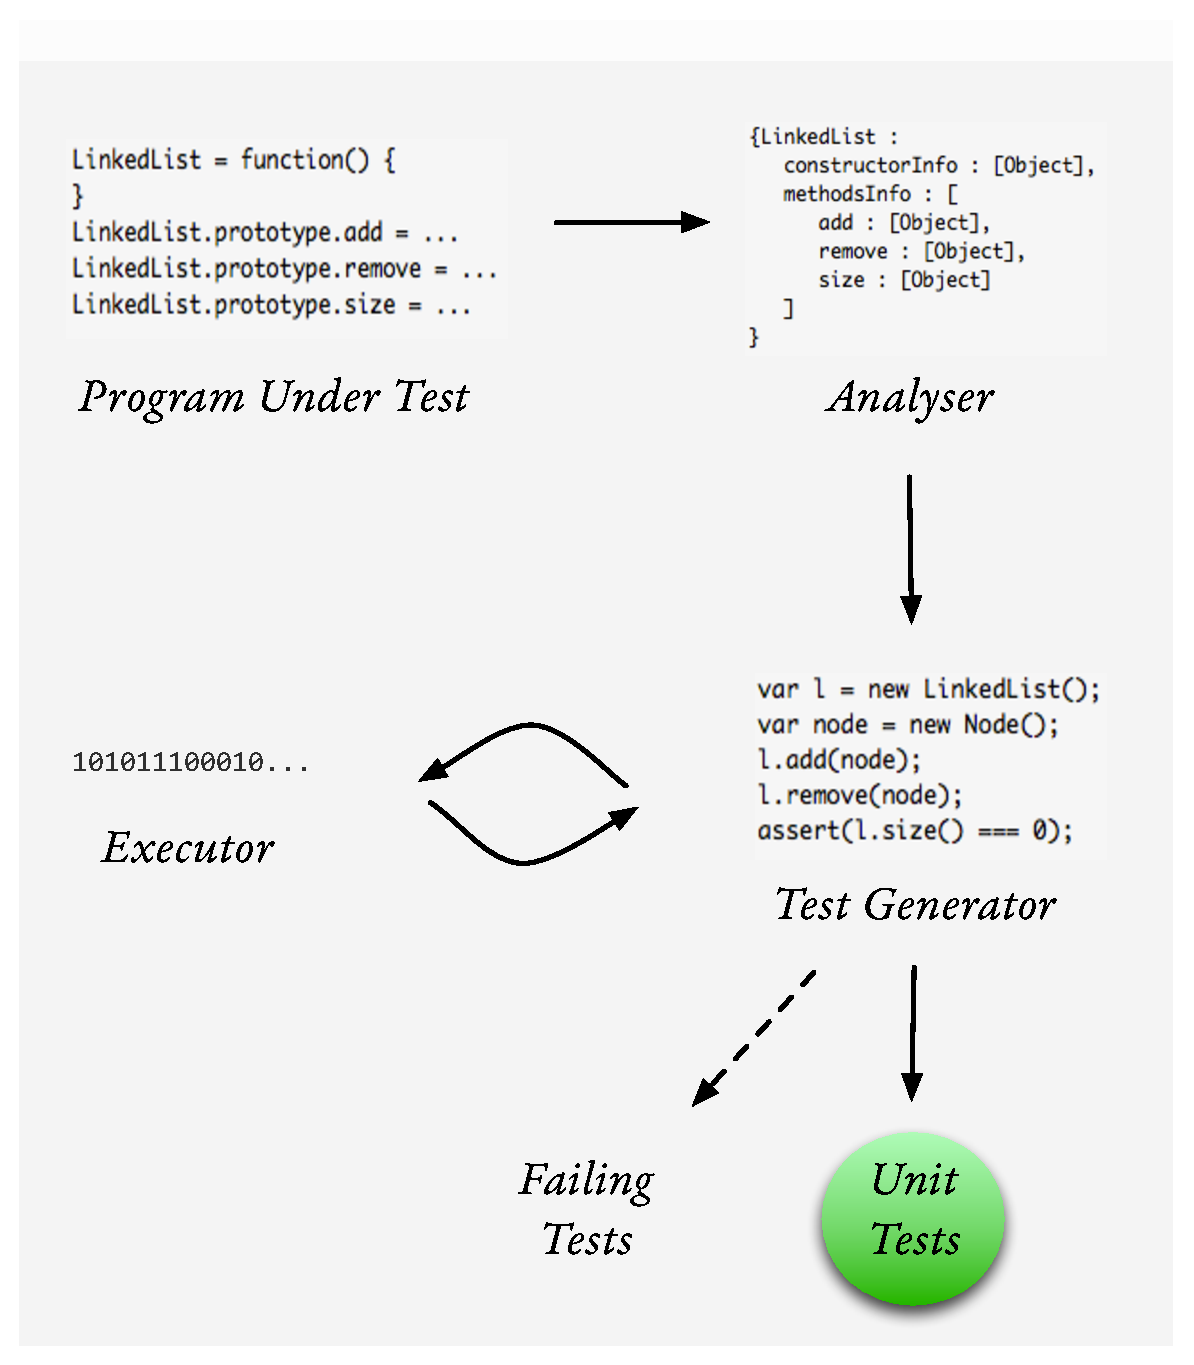
\includegraphics[scale=0.65]{./components/chapter3/system9.pdf}
\caption{The \textsf{Flycatcher} system}
\label{system}
\end{figure}